\documentclass{article}
\usepackage{fancyhdr}
\usepackage{tikz}
\usepackage{hyperref}
\usepackage{graphicx}
\usepackage{hyperref}

\pagestyle{fancy}
\fancyhf{}
\fancyhead[L]{\thepage}
\fancyhead[R]{\nouppercase{\leftmark}}


\newcommand{\mytikz}[1]{%
    \begin{figure}[ht]
        \centering
        #1
    \end{figure}
}

\begin{document}


\begin{titlepage}
    \centering
    \vspace*{\fill}
    \large{Computer Workshop \\
Final Assignment} \\

    \normalsize{Dr. Maleki Majd}
    \vspace*{\fill}
    \thispagestyle{empty}
\end{titlepage}



\tableofcontents
\clearpage

\section{1 Git and GitHub}
\subsection{ Repository Initialization and Commits}
I initialized the Git repository for this assignment using the following commands:
\begin{verbatim}
$ git init
$ git add .
$ git commit -m "Initialized repository for the final assignment."
\end{verbatim}

\subsection{GitHub Actions for LaTeX Compilation}
Create a new file named \texttt{.github/workflows/main.yml} in the root of your repository. This file will define the GitHub Actions workflow.
Open \texttt{main.yml} and add the following content:

\begin{verbatim}
name: Compile LaTeX

on:
  push:
    branches:
      - main

jobs:
  build:
    runs-on: ubuntu-latest

    steps:
    - name: Set up Git repository
      uses: actions/checkout@v2

    - name: Compile LaTeX
      run: pdflatex -interaction=nonstopmode -halt-on-error main.tex
\end{verbatim}

\section{Exploration Tasks}
\subsection{Vim Advanced Features}
\begin{enumerate}
    \item \textbf{Multiple Cursors:} Vim supports multiple cursors, allowing you to edit multiple occurrences of a word simultaneously. To use this feature:
    
    \begin{itemize}
        \item Place the cursor on a word.
        \item Press \texttt{Ctrl} + \texttt{D} to select the word under the cursor.
        \item Press \texttt{Ctrl} + \texttt{D} again to select the next occurrence.
        \item You can now edit all selected occurrences simultaneously.
    \end{itemize}

    \item \textbf{Window Resizing:} Vim allows you to resize split windows dynamically. To resize a split window:
    
    \begin{itemize}
        \item Press \texttt{Ctrl} + \texttt{W} and release.
        \item Press \texttt{>} to increase width or \texttt{<} to decrease width.
        \item Press \texttt{+} to increase height or \texttt{-} to decrease height.
    \end{itemize}

    \item \textbf{Vim Registers:} Registers in Vim allow you to yank and paste text selectively. Some advanced register usage includes:
    
    \begin{itemize}
        \item \texttt{"ayy}: Yank the current line into register \texttt{a}.
        \item \texttt{"ap}: Paste the contents of register \texttt{a}.
        \item \texttt{":p}: Paste from the system clipboard (requires Vim with clipboard support).
    \end{itemize}
\end{enumerate}

\subsection{Memory profiling}
\begin{enumerate}
    \item \textbf{Memory Leak:}
    
    In a program, a memory leak occurs when the program allocates memory dynamically (using functions like \texttt{malloc()} or \texttt{new}) but fails to release or deallocate that memory properly before the program terminates. This leads to a gradual accumulation of unused memory, and if the program runs for an extended period, it can eventually consume a significant amount of system memory. Memory leaks are a common source of performance issues and can cause programs to become slower or even crash.

    Memory leaks can happen due to various reasons, such as:

    \begin{itemize}
        \item Forgetting to free allocated memory using \texttt{free()} or \texttt{delete}.
        \item Losing track of pointers that point to allocated memory.
        \item Failing to release memory in error or exceptional conditions.
    \end{itemize}

    Detecting and fixing memory leaks is crucial for writing robust and efficient software.

    \item \textbf{Memory Profilers:}

    Memory profilers are tools designed to help developers identify and analyze memory-related issues in their programs. One such powerful tool is \textbf{Valgrind}.

    \textbf{Valgrind} is a programming tool suite that provides various tools for memory profiling, including a memory leak detector. Its purpose is to assist developers in finding memory leaks, memory corruption, and other memory-related errors in C and C++ programs.

    How Valgrind helps when memory leaks happen:

    \begin{itemize}
        \item **Memory Leak Detection:** Valgrind can detect memory leaks by tracking memory allocations and deallocations during program execution. It reports any memory that was allocated but not freed.

        \item **Memory Error Detection:** Valgrind can identify memory-related errors such as accessing uninitialized memory, using memory after it has been freed, and other memory corruption issues.

        \item **Call Graphs and Profiling:** Valgrind provides detailed information about the program's memory usage, allowing developers to analyze memory behavior and optimize their code.

        \item **Dynamic Analysis:** Valgrind uses dynamic binary instrumentation to intercept memory-related function calls, providing a comprehensive view of memory usage during runtime.
    \end{itemize}

    By using Valgrind, developers can gain insights into the memory behavior of their programs, identify potential issues, and ensure efficient memory management.
\end{enumerate}


\subsection{GNU/Linux Bash Scripting}
\begin{enumerate}
    \item \textbf{2.3.1 fzf:}
    
    \begin{itemize}
        \item \textbf{Fuzzy Searching:} Fuzzy searching is a technique that matches approximate patterns rather than exact ones. It allows finding results that are similar but not identical to the search query.

        \item \textbf{Install fzf:} The command \texttt{ls | fzf} lists the files in the current directory and uses fzf for interactive, fuzzy selection. The selected file is then displayed on the terminal.
    \end{itemize}

    \item \textbf{2.3.2 Using fzf to find your favorite PDF:}
    
    \begin{enumerate}
        \item \textbf{List PDF files:} The command to list all files with the extension .PDF in the current directory is:
        
        \texttt{find . -name "*.PDF"}

        \item \textbf{Select PDF with fzf:} The command to use fzf for selecting a PDF from the list is:
        
        \texttt{find . -name "*.PDF" | fzf}
    \end{enumerate}

    \item \textbf{2.3.3 Opening the file using Zathura:}

    To open the selected PDF using Zathura, the command would be:

    \texttt{zathura \$(find . -name "*.PDF" | fzf)}
    
    
\section{Git and FOSS}


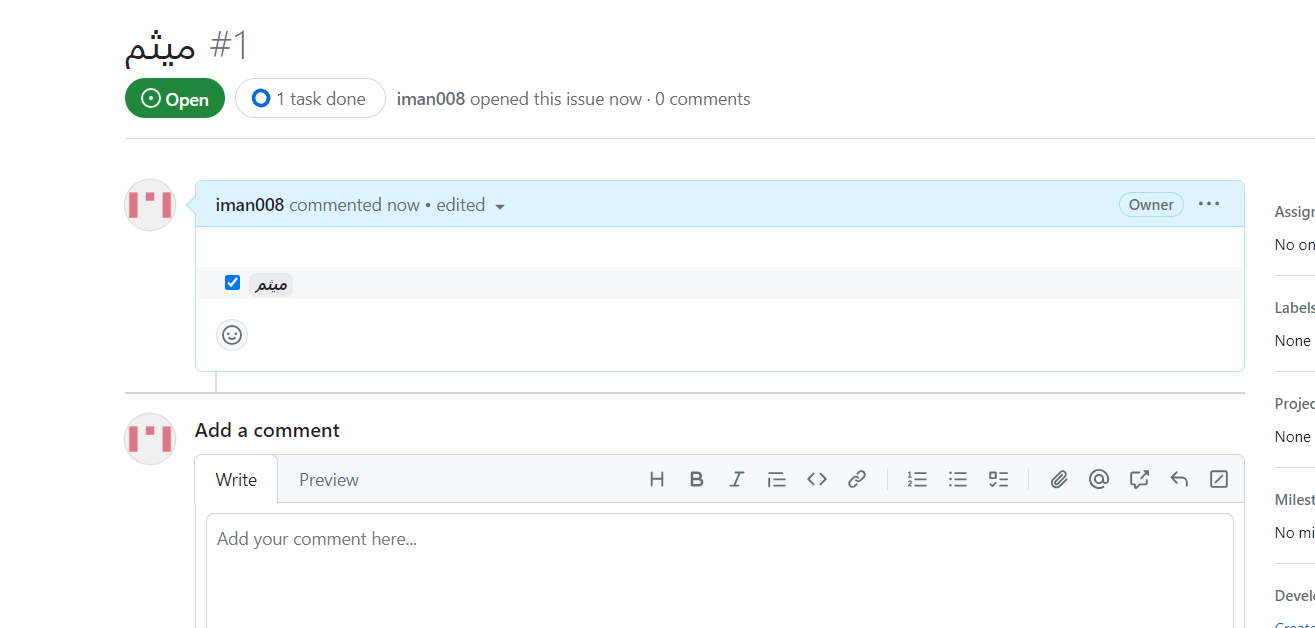
\includegraphics[width=0.8\textwidth]{meysam.png}\\
the link to github repo: \url{https://github.com/iman008/ComputerLabFinalAssignment}.




\end{enumerate}

\end{document}

















